\section{Smoothing}

\textbf{(a)}
The convolution matrix is
\[
A_{ij}=
\begin{cases}
c_{j-i},&-h\leq j-i\leq h\\
0,&\text{otherwise}
\end{cases}
\]
where entries outside the signal are omitted. Then
\[
y=Ax+w
\]
For the data, \(n=200\) and \(h=20\). The singular values decay from
\[
\sigma_{\max}(A)=0.998929
\]
to
\[
\sigma_{\min}(A)=2.40405\times10^{-9}
\]

\begin{figure}[H]
    \centering
    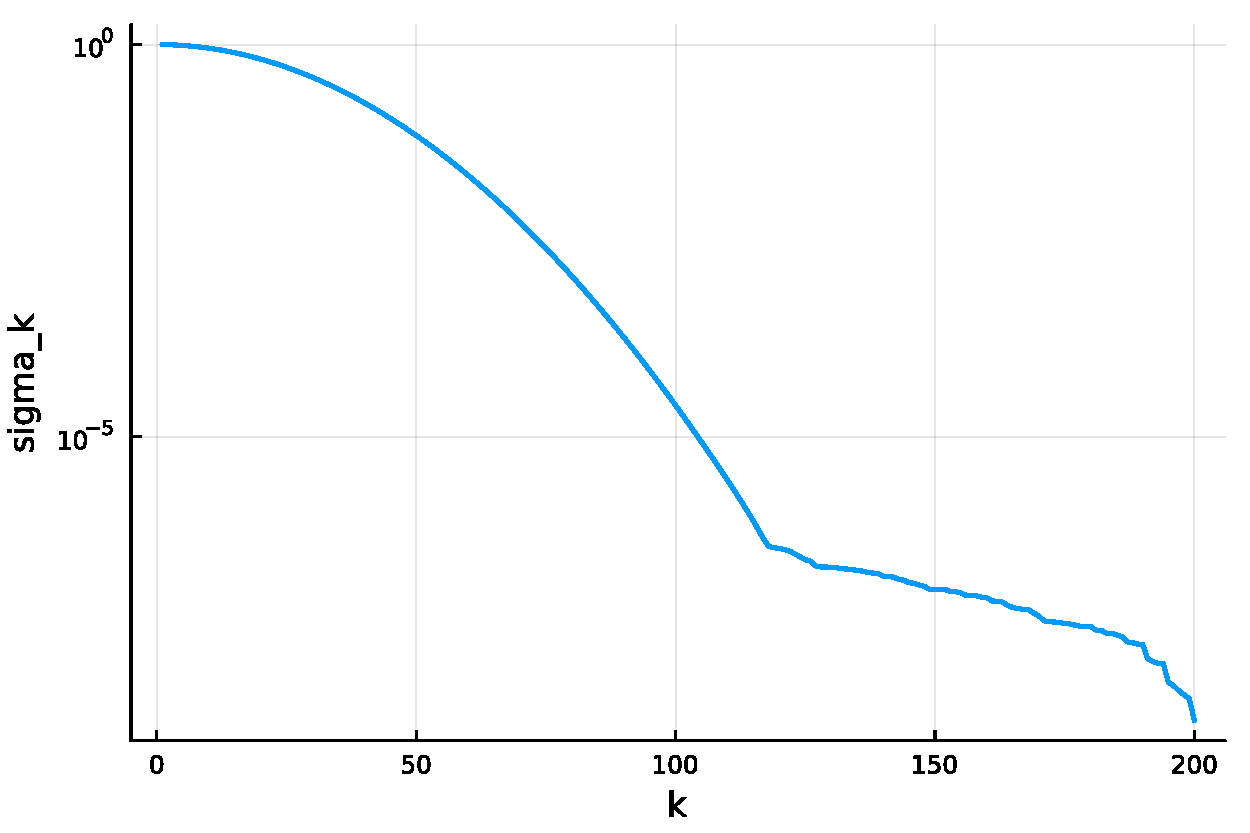
\includegraphics[width=0.78\textwidth]{img/p5_singular_values.pdf}
    % % \caption{Singular values of the convolution matrix on a logarithmic scale}
\end{figure}

\textbf{(b)}
The first six right singular vectors are smooth, oscillatory signals. The
first has almost no oscillation, and each subsequent vector has a higher
frequency. This is expected because convolution by the smooth kernel preserves
low-frequency directions most strongly, so they correspond to the largest
singular values.

\begin{figure}[H]
    \centering
    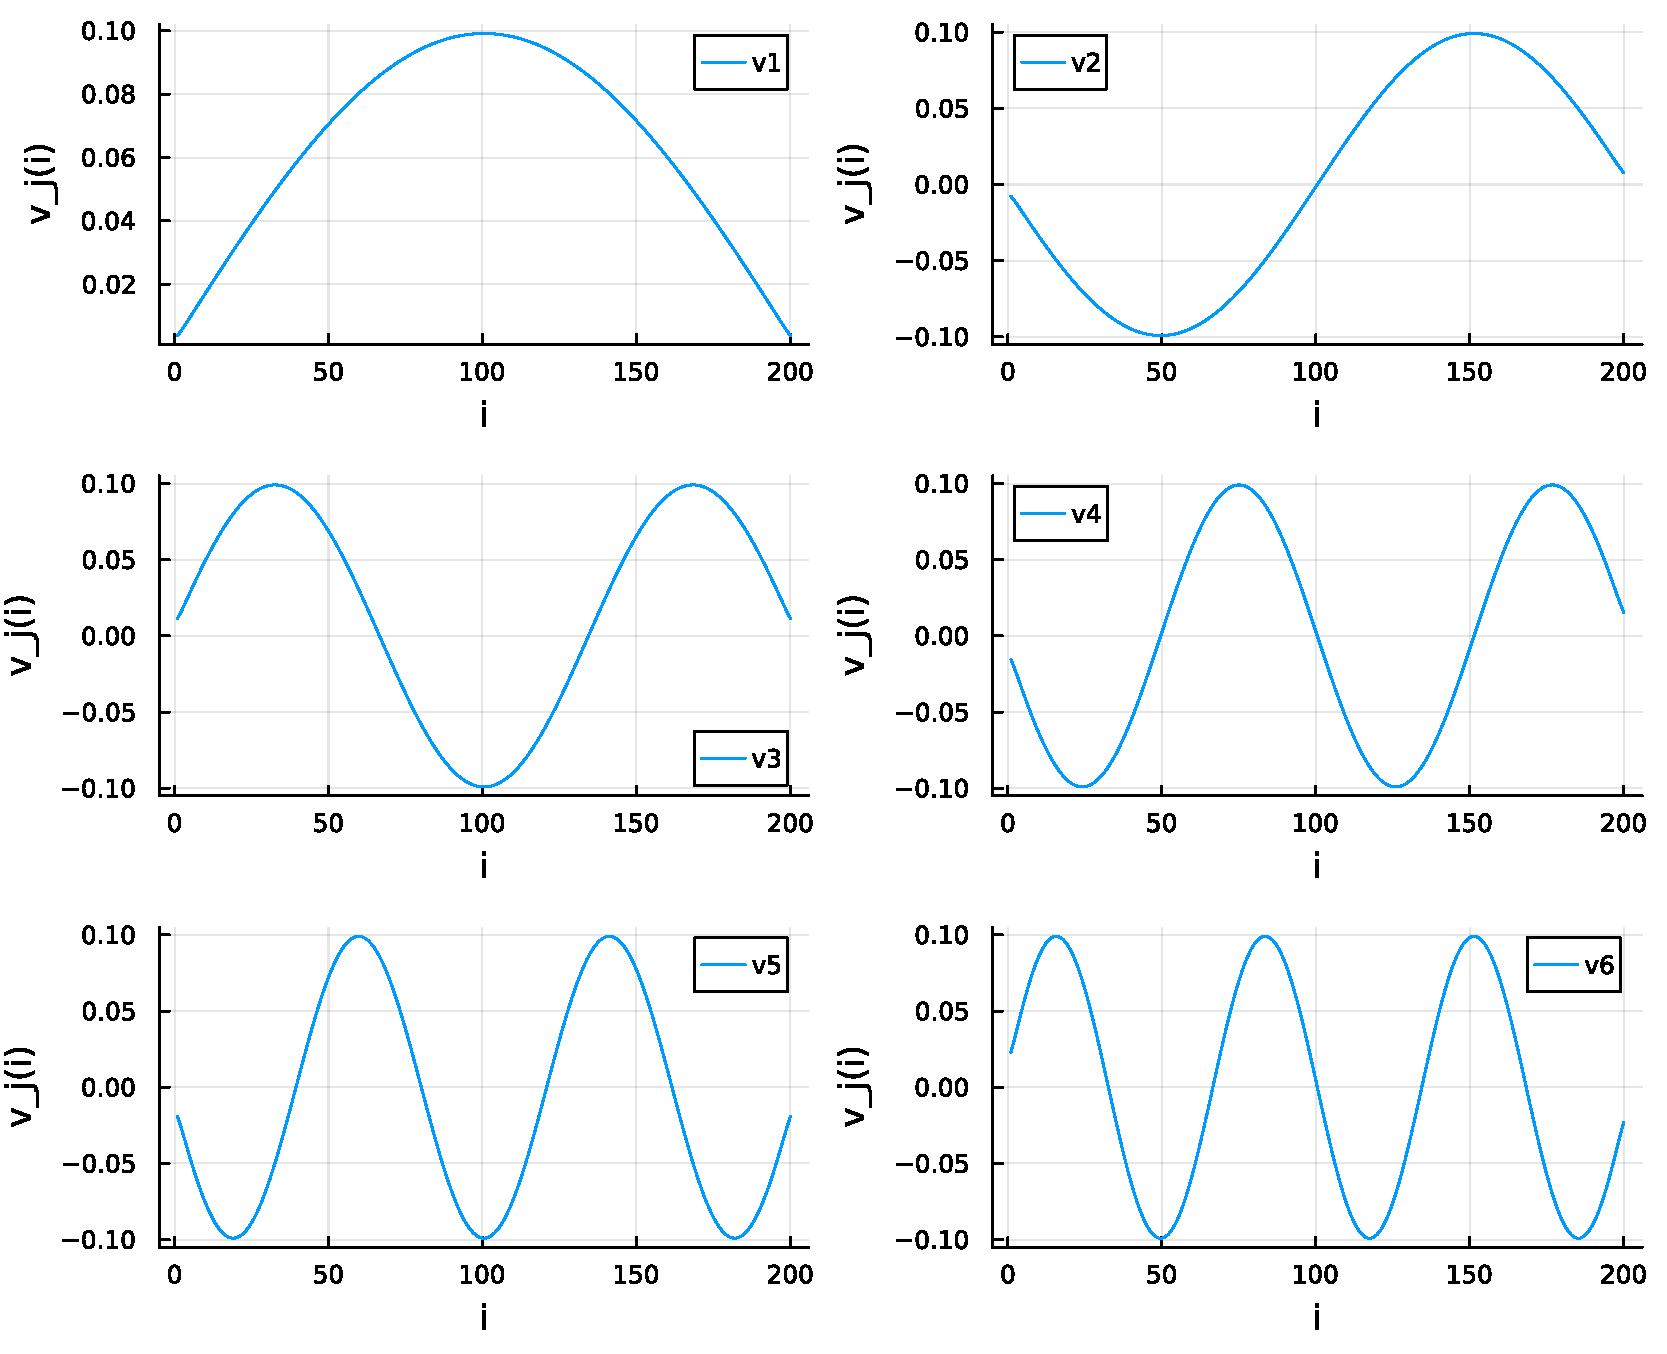
\includegraphics[width=\textwidth]{img/p5_right_vectors.pdf}
    \caption{First six right singular vectors}
\end{figure}

\textbf{(c)}
The condition number is
\[
\kappa(A)
=\frac{\sigma_{\max}(A)}{\sigma_{\min}(A)}
=4.15520\times10^8
\]
Writing \(A=U\Sigma V^T\), the least-squares estimate contains terms
\[
\frac{u_i^Ty_{\mathrm{meas}}}{\sigma_i}v_i
\]
Thus noise in directions with very small \(\sigma_i\) is amplified enormously.
The resulting error is
\[
\|x-x_{\mathrm{ls}}\|_2=2.34098\times10^8
\]

\begin{figure}[H]
    \centering
    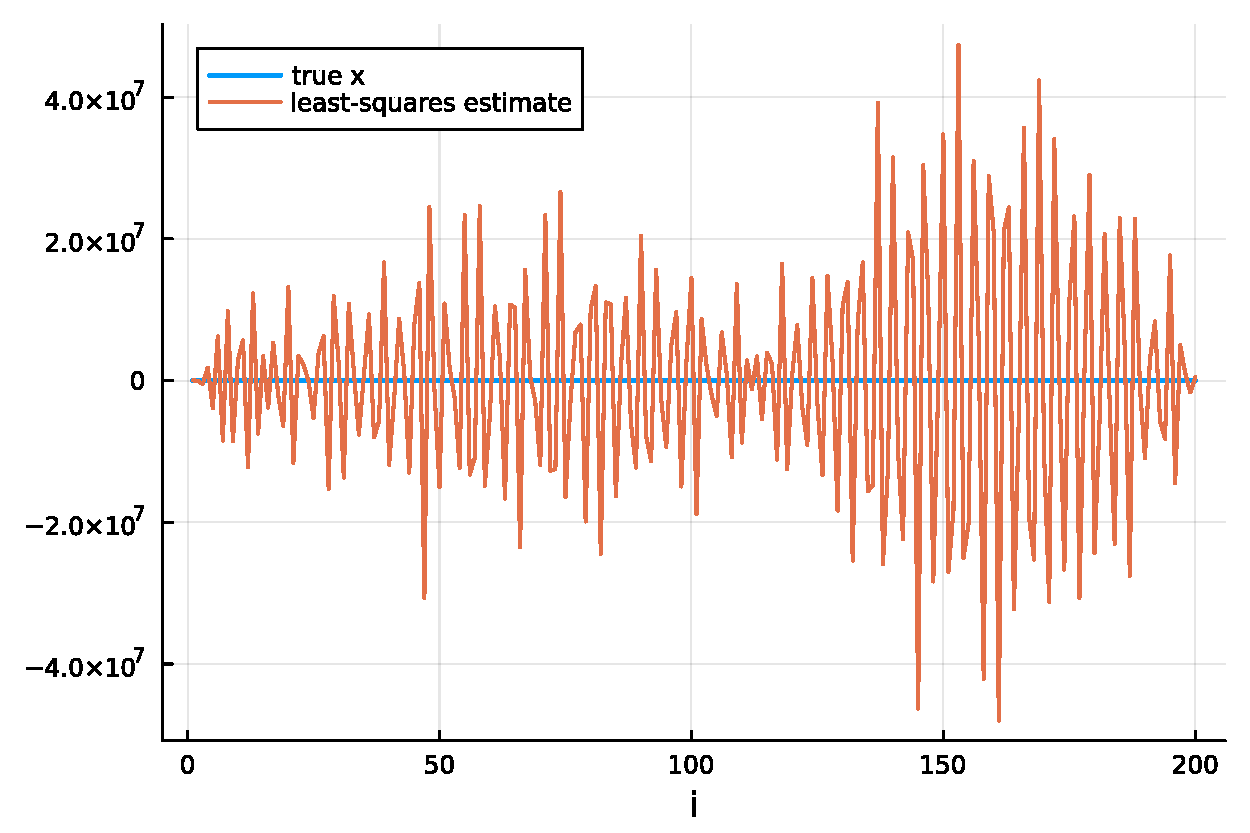
\includegraphics[width=0.82\textwidth]{img/p5_least_squares.pdf}
    \caption{Unregularized least-squares estimate}
\end{figure}

\textbf{(d)}
For rank \(r\), the truncated estimate is
\[
x_{\mathrm{est}}^{(r)}
=V_r\Sigma_r^{-1}U_r^Ty_{\mathrm{meas}}
\]
The observed errors for the requested ranks are
\[
\begin{array}{c|ccccc}
r&5&10&15&30&50\\ \hline
\|x-x_{\mathrm{est}}^{(r)}\|_2
&20.662&16.346&12.819&10.604&15.177
\end{array}
\]
Small \(r\) gives an overly smooth estimate. Increasing \(r\) initially
recovers the transitions in \(x\), but at \(r=50\) more noise-dominated
directions enter and the estimate becomes oscillatory.

\begin{figure}[H]
    \centering
    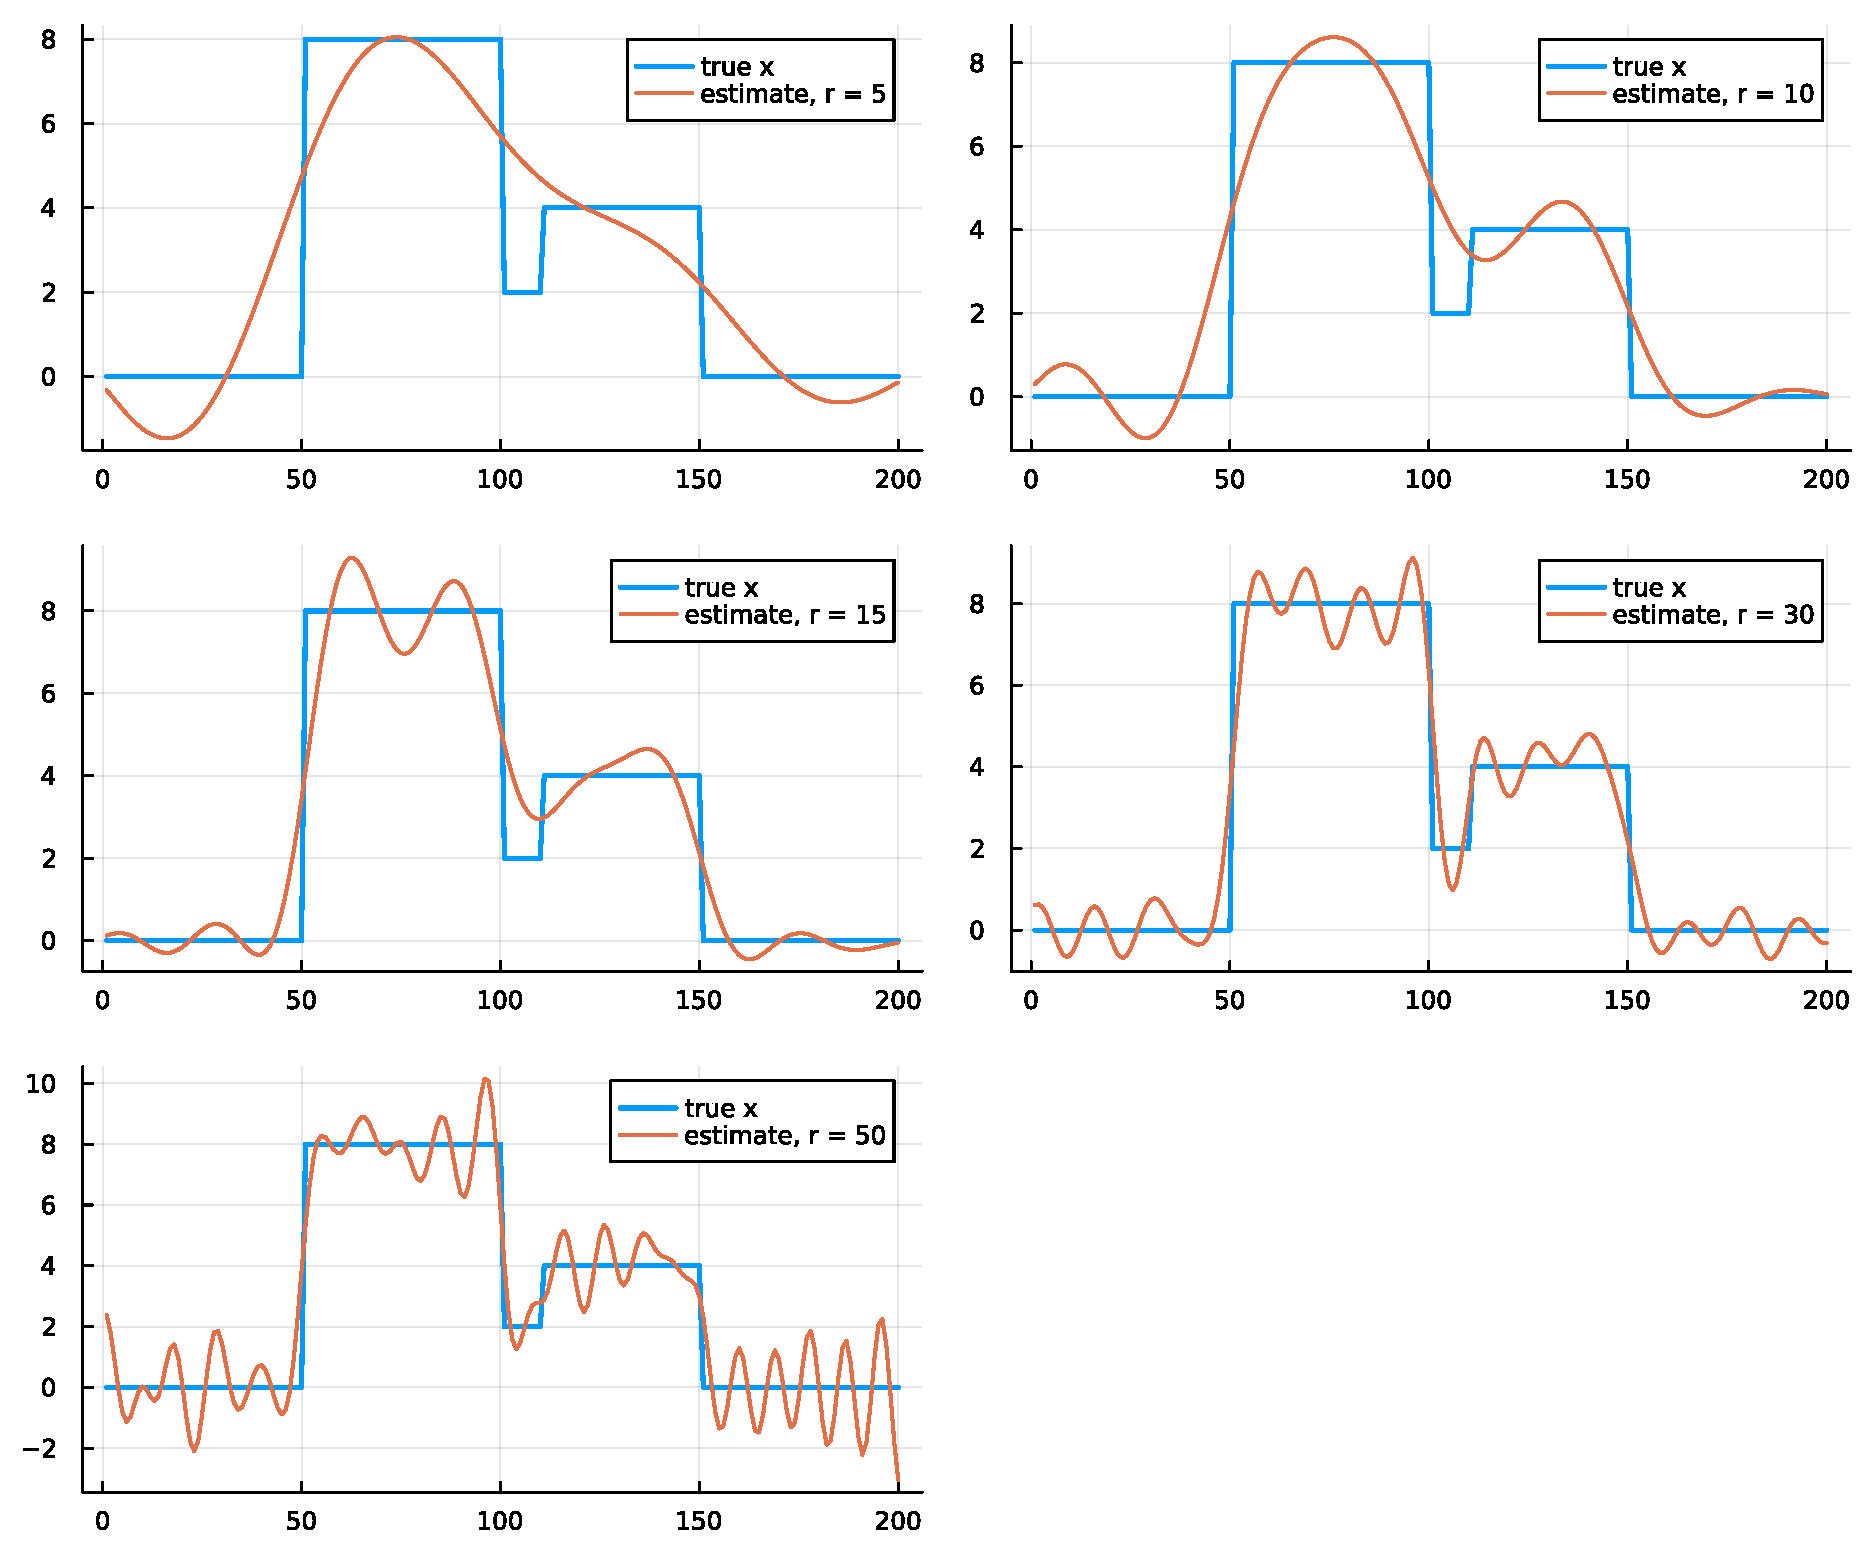
\includegraphics[width=\textwidth]{img/p5_truncated_estimates.pdf}
    % \caption{Truncated-SVD estimates for several ranks}
\end{figure}

\textbf{(e)}
The error decreases as useful singular-vector components are added, reaches
its minimum at \(r=28\), and then begins to increase as noise amplification
outweighs the added signal information.

\begin{figure}[H]
    \centering
    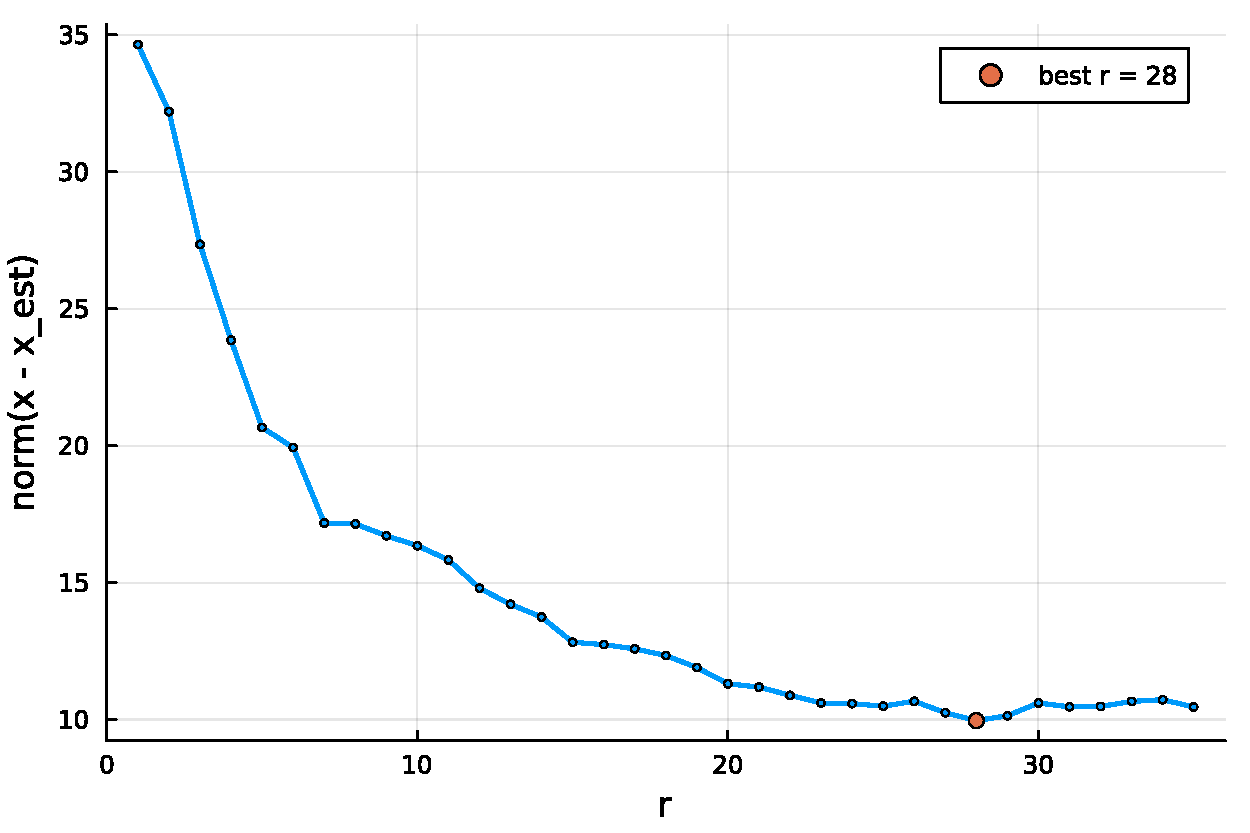
\includegraphics[width=0.78\textwidth]{img/p5_truncation_error.pdf}
    % \caption{Truncated-SVD estimation error}
\end{figure}

\textbf{(f)}
Among \(r=1,\ldots,35\), the best value is
\[
\boxed{r=28}
\]
with error
\[
\|x-x_{\mathrm{est}}^{(28)}\|_2=9.95897
\]

\begin{figure}[H]
    \centering
    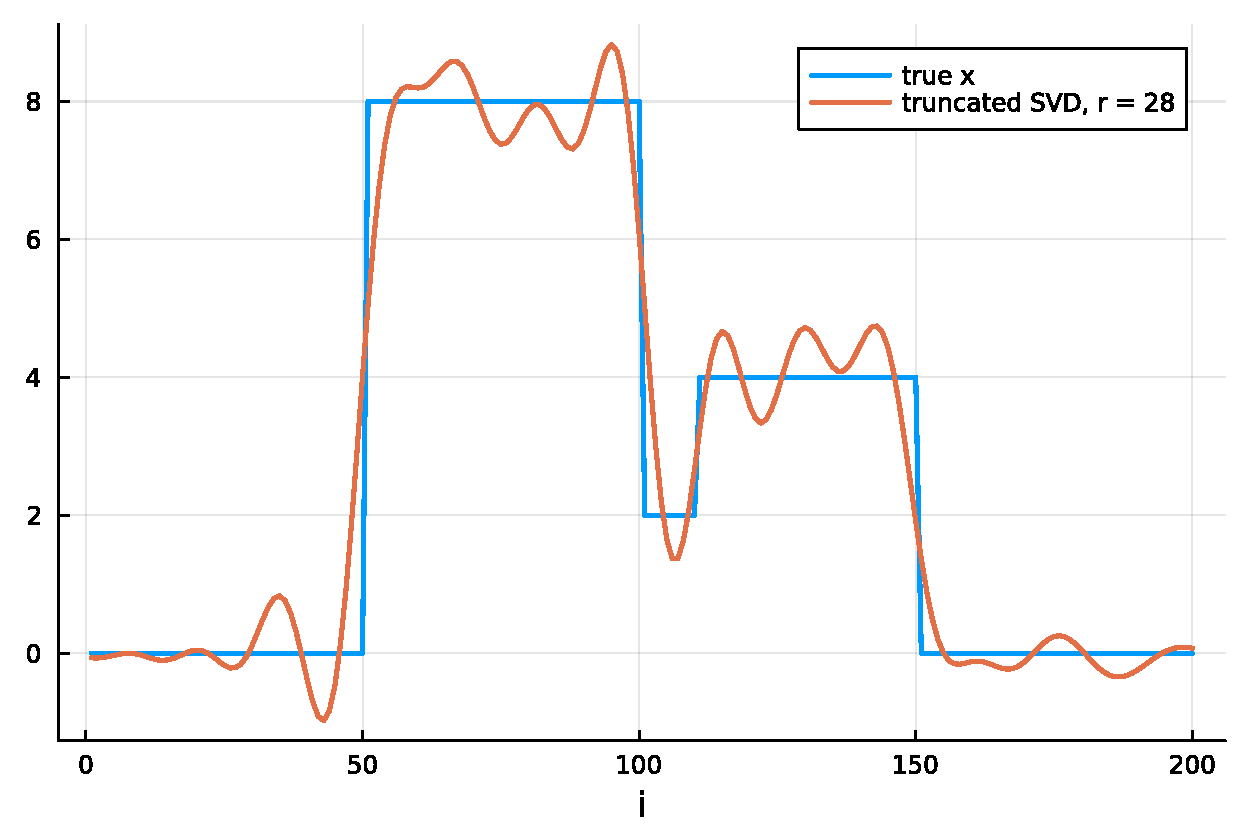
\includegraphics[width=0.82\textwidth]{img/p5_best_truncated.pdf}
    % \caption{Best truncated-SVD estimate}
\end{figure}

\textbf{(g)}
The Tikhonov objective is
\[
% J(x)=\|Ax-y_{\mathrm{meas}}\|_2^2+\mu\|x\|_2^2
J(x)=\|Ax-y\|^2+\mu\|x\|^2
\]
Setting its gradient to zero gives
\[
(A^TA+\mu I)x_{\mathrm{reg}}=A^Ty_{\mathrm{meas}}
\]
and therefore
\[
\boxed{x_{\mathrm{reg}}
=(A^TA+\mu I)^{-1}A^Ty_{\mathrm{meas}}}
\]
% Scanning a logarithmic range of parameters gives a good estimate at
There is a good estimate at
\[
\mu=0.05012
\]
with error \(9.95345\).

\begin{figure}[H]
    \centering
    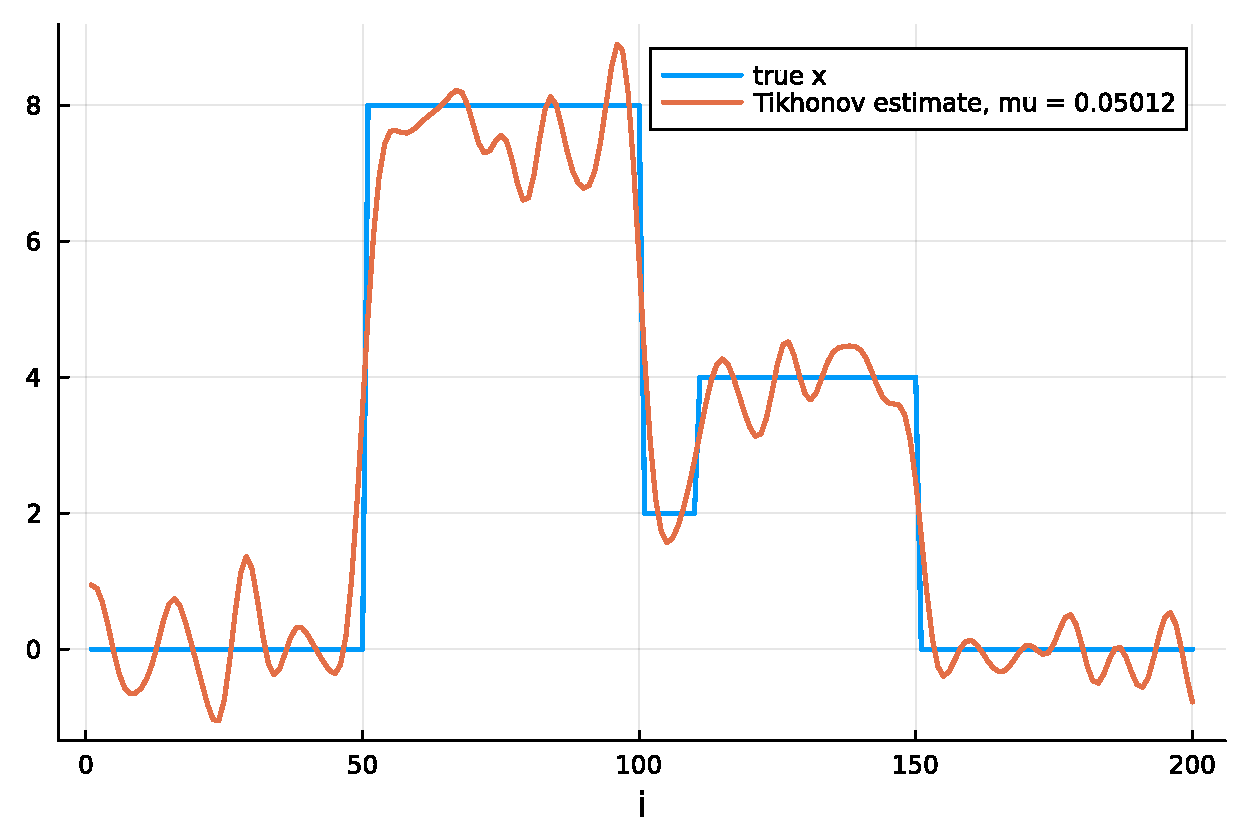
\includegraphics[width=0.82\textwidth]{img/p5_tikhonov.pdf}
    % \caption{Tikhonov-regularized estimate}
\end{figure}

\textbf{(h)}
Let
\[
A=U\Sigma V^T
=\sum_{i=1}^n\sigma_i u_i v_i^T
\]
Then
\[
B=(A^TA+\mu I)^{-1}A^T
=V\operatorname{diag}\left(
\frac{\sigma_i}{\sigma_i^2+\mu}\right)U^T
\]
Define
\[
g_i=\frac{\sigma_i}{\sigma_i^2+\mu}
\]
These gains are not necessarily sorted when the \(\sigma_i\) are sorted. Let
\(\pi\) order them so that
\[
g_{\pi(1)}\geq\cdots\geq g_{\pi(n)}
\]
Then the SVD of \(B\) is obtained from
\[
\boxed{
\widetilde\sigma_j=g_{\pi(j)},\qquad
\widetilde u_j=v_{\pi(j)},\qquad
\widetilde v_j=u_{\pi(j)}
}
\]

\textbf{(i)}
The norm of \(B\) is its largest singular value:
\[
\boxed{\|B\|_2
=\max_i\frac{\sigma_i}{\sigma_i^2+\mu}}
\]
For the selected \(\mu\), this is approximately \(2.23226\).

\textbf{(j)}
Using the SVD,
\[
AB
=U\operatorname{diag}\left(
\frac{\sigma_i^2}{\sigma_i^2+\mu}\right)U^T
\]
so
\[
AB-I
=-U\operatorname{diag}\left(
\frac{\mu}{\sigma_i^2+\mu}\right)U^T
\]
Therefore
\[
\boxed{
\max_{y\neq0}\frac{\|ABy-y\|_2}{\|y\|_2}
=\|AB-I\|_2
=\max_i\frac{\mu}{\sigma_i^2+\mu}
=\frac{\mu}{\sigma_{\min}(A)^2+\mu}
}
\]
For the selected \(\mu\), this value is numerically \(1.00000\), since the
smallest singular value is extremely close to zero.

\subsection{Code}
\begin{lstlisting}[language={}]
using LinearAlgebra
using Plots

include(joinpath(@__DIR__, "readclassjson.jl"))
data = readclassjson(joinpath(@__DIR__, "regl_data.json"))
n, c = data["n"], data["c"]
x, w = vec(data["x"]), vec(data["w"])

function convolution_matrix(c, n)
    h = div(length(c) - 1, 2)
    A = zeros(n, n)
    for i in 1:n, k in -h:h
        j = i + k
        if 1 <= j <= n
            A[i, j] = c[k + h + 1]
        end
    end
    return A
end

A = convolution_matrix(c, n)
ymeas = A * x + w
F = svd(A)

plot(1:n, F.S; yscale=:log10,
     xlabel="k", ylabel="sigma_k")
plot(1:n, F.V[:, 1:6]; layout=(3, 2))

xls = A \ ymeas
p_ls = plot(x; label="true x")
plot!(p_ls, xls; label="least-squares estimate")

function truncated_estimate(F, y, r)
    Ur = F.U[:, 1:r]
    Vr = F.V[:, 1:r]
    return Vr * ((Ur' * y) ./ F.S[1:r])
end

ranks = [5, 10, 15, 30, 50]
xtruncated = [
    truncated_estimate(F, ymeas, r) for r in ranks
]
rank_plots = map(zip(ranks, xtruncated)) do (r, xr)
    p = plot(x; label="true x")
    plot!(p, xr; label="estimate, r = $r")
end
plot(rank_plots...; layout=(3, 2))

tested_ranks = 1:35
rank_errors = [
    norm(x - truncated_estimate(F, ymeas, r))
    for r in tested_ranks
]
best_r = tested_ranks[argmin(rank_errors)]
plot(tested_ranks, rank_errors;
     xlabel="r", ylabel="norm(x - x_est)")
xbest = truncated_estimate(F, ymeas, best_r)
p_best = plot(x; label="true x")
plot!(p_best, xbest; label="best truncated estimate")

function tikhonov_estimate(F, y, mu)
    gains = F.S ./ (F.S .^ 2 .+ mu)
    return F.V * (gains .* (F.U' * y))
end

mus = 10.0 .^ range(-10, 0; length=301)
reg_errors = [
    norm(x - tikhonov_estimate(F, ymeas, mu))
    for mu in mus
]
best_mu = mus[argmin(reg_errors)]
xreg = tikhonov_estimate(F, ymeas, best_mu)
p_reg = plot(x; label="true x")
plot!(p_reg, xreg; label="Tikhonov estimate")
\end{lstlisting}
